\subsection{RVAgene modeling of pseudotemporally ordered data during embryonic stem cell differentiation}

We applied RVAgene to model gene expression dynamics during embryonic stem cell (ESC) differentiation. \citet{Klein2015} identified 732 differentially expressed genes over the time course of mouse ESC differentiation following leukemia inhibitory factor (LIF) withdrawal. Data is gathered at four time points: 0, 2, 4, and 7 days after LIF withdrawal. (Table S2 in \citet{Klein2015}). We ordered the data (2717 single cells) using diffusion pseudotime (DPT), which provides robust methods for the reconstruction of single-cell temporal processes \citep{haghverdi2016diffusion}. The root cell was randomly sampled from the initial time point (\hyperref[fig:fig3]{Fig. 2A}). The inferred pseudotime is highly correlated with the experimental time points, giving confidence that true biological processes are represented over the DPT pseudotime. The gene expression dynamics over pseudotime show considerable variability among cells. To smooth the data, we apply a moving window average, over windows of length 40, to give 68 time points after smoothing (\hyperref[fig:fig3]{Fig. 2A}). 
We fit linear regression models to the smoothed pseudotime profiles of each gene (\hyperref[supp]{Fig. S2}), and see that for the majority of genes the correlation coefficients are $> 0.5$ (\hyperref[fig:fig3]{Fig. 2B}), with a clear distinction between the up- and down-regulated genes over pseudotime.
\par 
An RVAgene model was trained on the data with a two-dimensional latent space, on which genes are classified based on their correlation coefficients  (\hyperref[fig:fig3]{Fig. 2C}). Two distinctive characteristics emerge: a) the two groups (up- and down-regulated genes) are well-separated in the latent space, and b) the two groups merge and overlap at some point, illustrating the continuity of the latent space, as discussed above. 
We compared the results of RVAgene with DPGP, an unsupervised approach for gene expression time series clustering \citep{McDowell2018}. DPGP is a hierarchical Bayesian model that estimates the number of clusters along with the cluster membership.

To assess the correspondence between methods, genes clustered by DPGP (\hyperref[supp]{Fig. S3}) were projected onto the RVAgene latent space (\hyperref[fig:fig3]{Fig. 2D}). Of the 12 clusters detected by DPGP, the four largest can be characterized by their up- and down-regulation profiles over pseudotime. On the RVAgene latent space, we find that genes sampled from each of the DPGP clusters appear close together, and moreover, are represented on a spectrum from upregulation to downregulation (\hyperref[fig:fig3]{Fig. 2D}). The goals of RVAgene and DPGP are to some degree complementary: DPGP characterizes gene expression profiles discretely with no need for prior information, while RVAgene characterizes profiles with a continuous representation, that can explain smooth changes in patterns.

%DPGP is a hierarchical Bayesian model that estimates the number of clusters along with the cluster membership, and outputs a posterior mean function and covariance matrix for each gene cluster. In contrast to RVAgene, DPGP does not assume any structure in gene expression data, performing an agnostic search, resulting in higher resource consumption (see \hyperref[supp]{Fig. S1}). DPGP does perform unsupervised clustering, a key advantage, although it does not provide inter-cluster information or predictions, which are provided by RVAgene.


{\centering
\begin{figure}%\begin{wrapfigure}[19]{r}{75mm}
  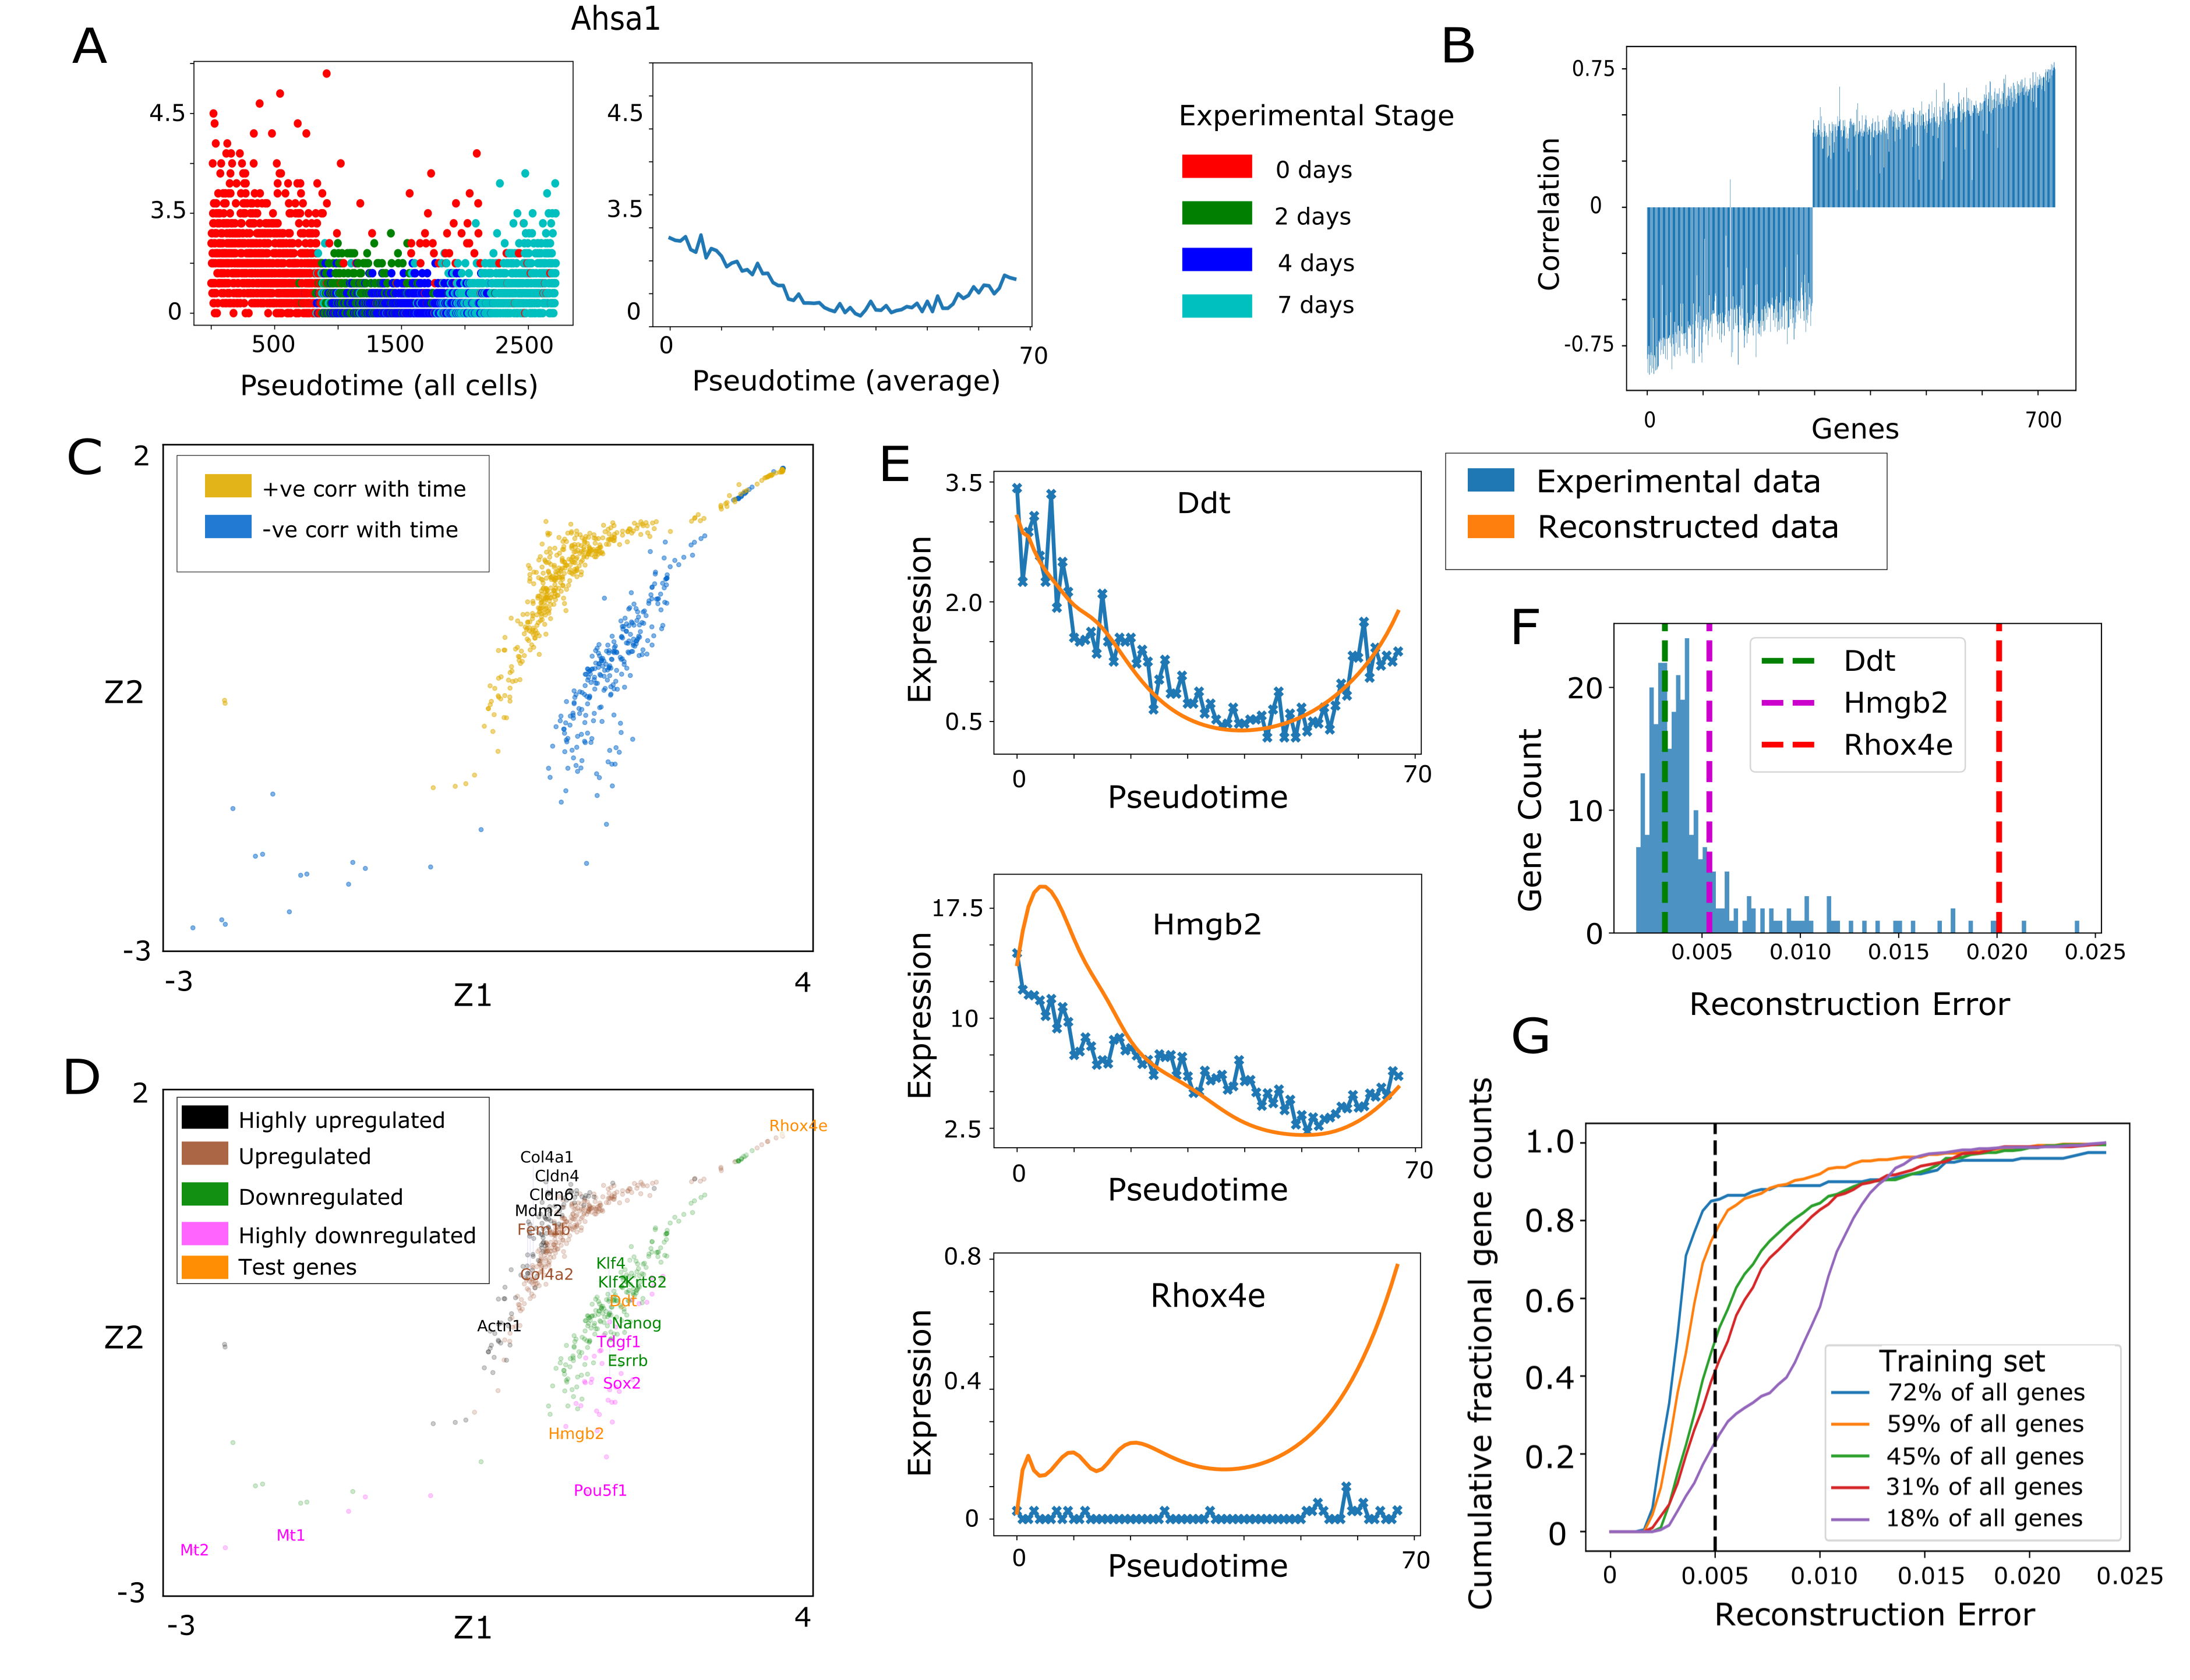
\includegraphics[width=\linewidth]{figures/esc_results.png}
 % archetecture.png: 1149x508 px, 72dpi, 40.53x17.92 cm, bb=0 0 1149 508
    \caption[Accurate reconstruction of embryonic stem cell differentiation dynamics with RVAgene.]{\textbf{Accurate reconstruction of embryonic stem cell differentiation dynamics with RVAgene.}
     ({\bf A}) Pseudotemporal ordering of 2717 single cells (data from \citep{Klein2015}), calculated using DPT; example gene shown: Ahsa1. Gene expression values given as log2(counts+1) for all cells (left), and for sliding window average (right).  ({\bf B}) Pearson correlation coefficient between gene expression and time for 732 differentially expressed genes.
    ({\bf C}) The 2D latent space learnt by an RVAgene model trained on 732 gene profiles over pseudotime, showing clear separation between upregulated and downregulated genes. ({\bf D}) Comparison of RVAgene and DPGP. The four largest clusters from DPGP are plotted on the RVAgene latent space: temporal expression patterns (from highly upregulated to highly downregulated) are in close agreement between methods. ({\bf E}) Comparison of experimental data and reconstructions. Model-generated reconstructions of three genes from the test set not used in training: Ddt, Hmgb2, and Rhox4e. Expression values are log2(counts+1).
    ({\bf F}) Distribution of average $L1$ reconstruction errors for the 300 genes used in the test set. Genes plotted in C are marked.
    ({\bf G}) Cumulative distributions of reconstruction errors on randomly sampled sets of test genes, where the full data were split into test groups of: 200 genes (train on 72\%), 300 genes (train on 59\%), 400 genes (train on 45\%), 500 genes (train on 31\%), and 600 genes (train on 18\%).}
    \label{fig:fig3}
\end{figure}
}

{\centering
\begin{figure}
  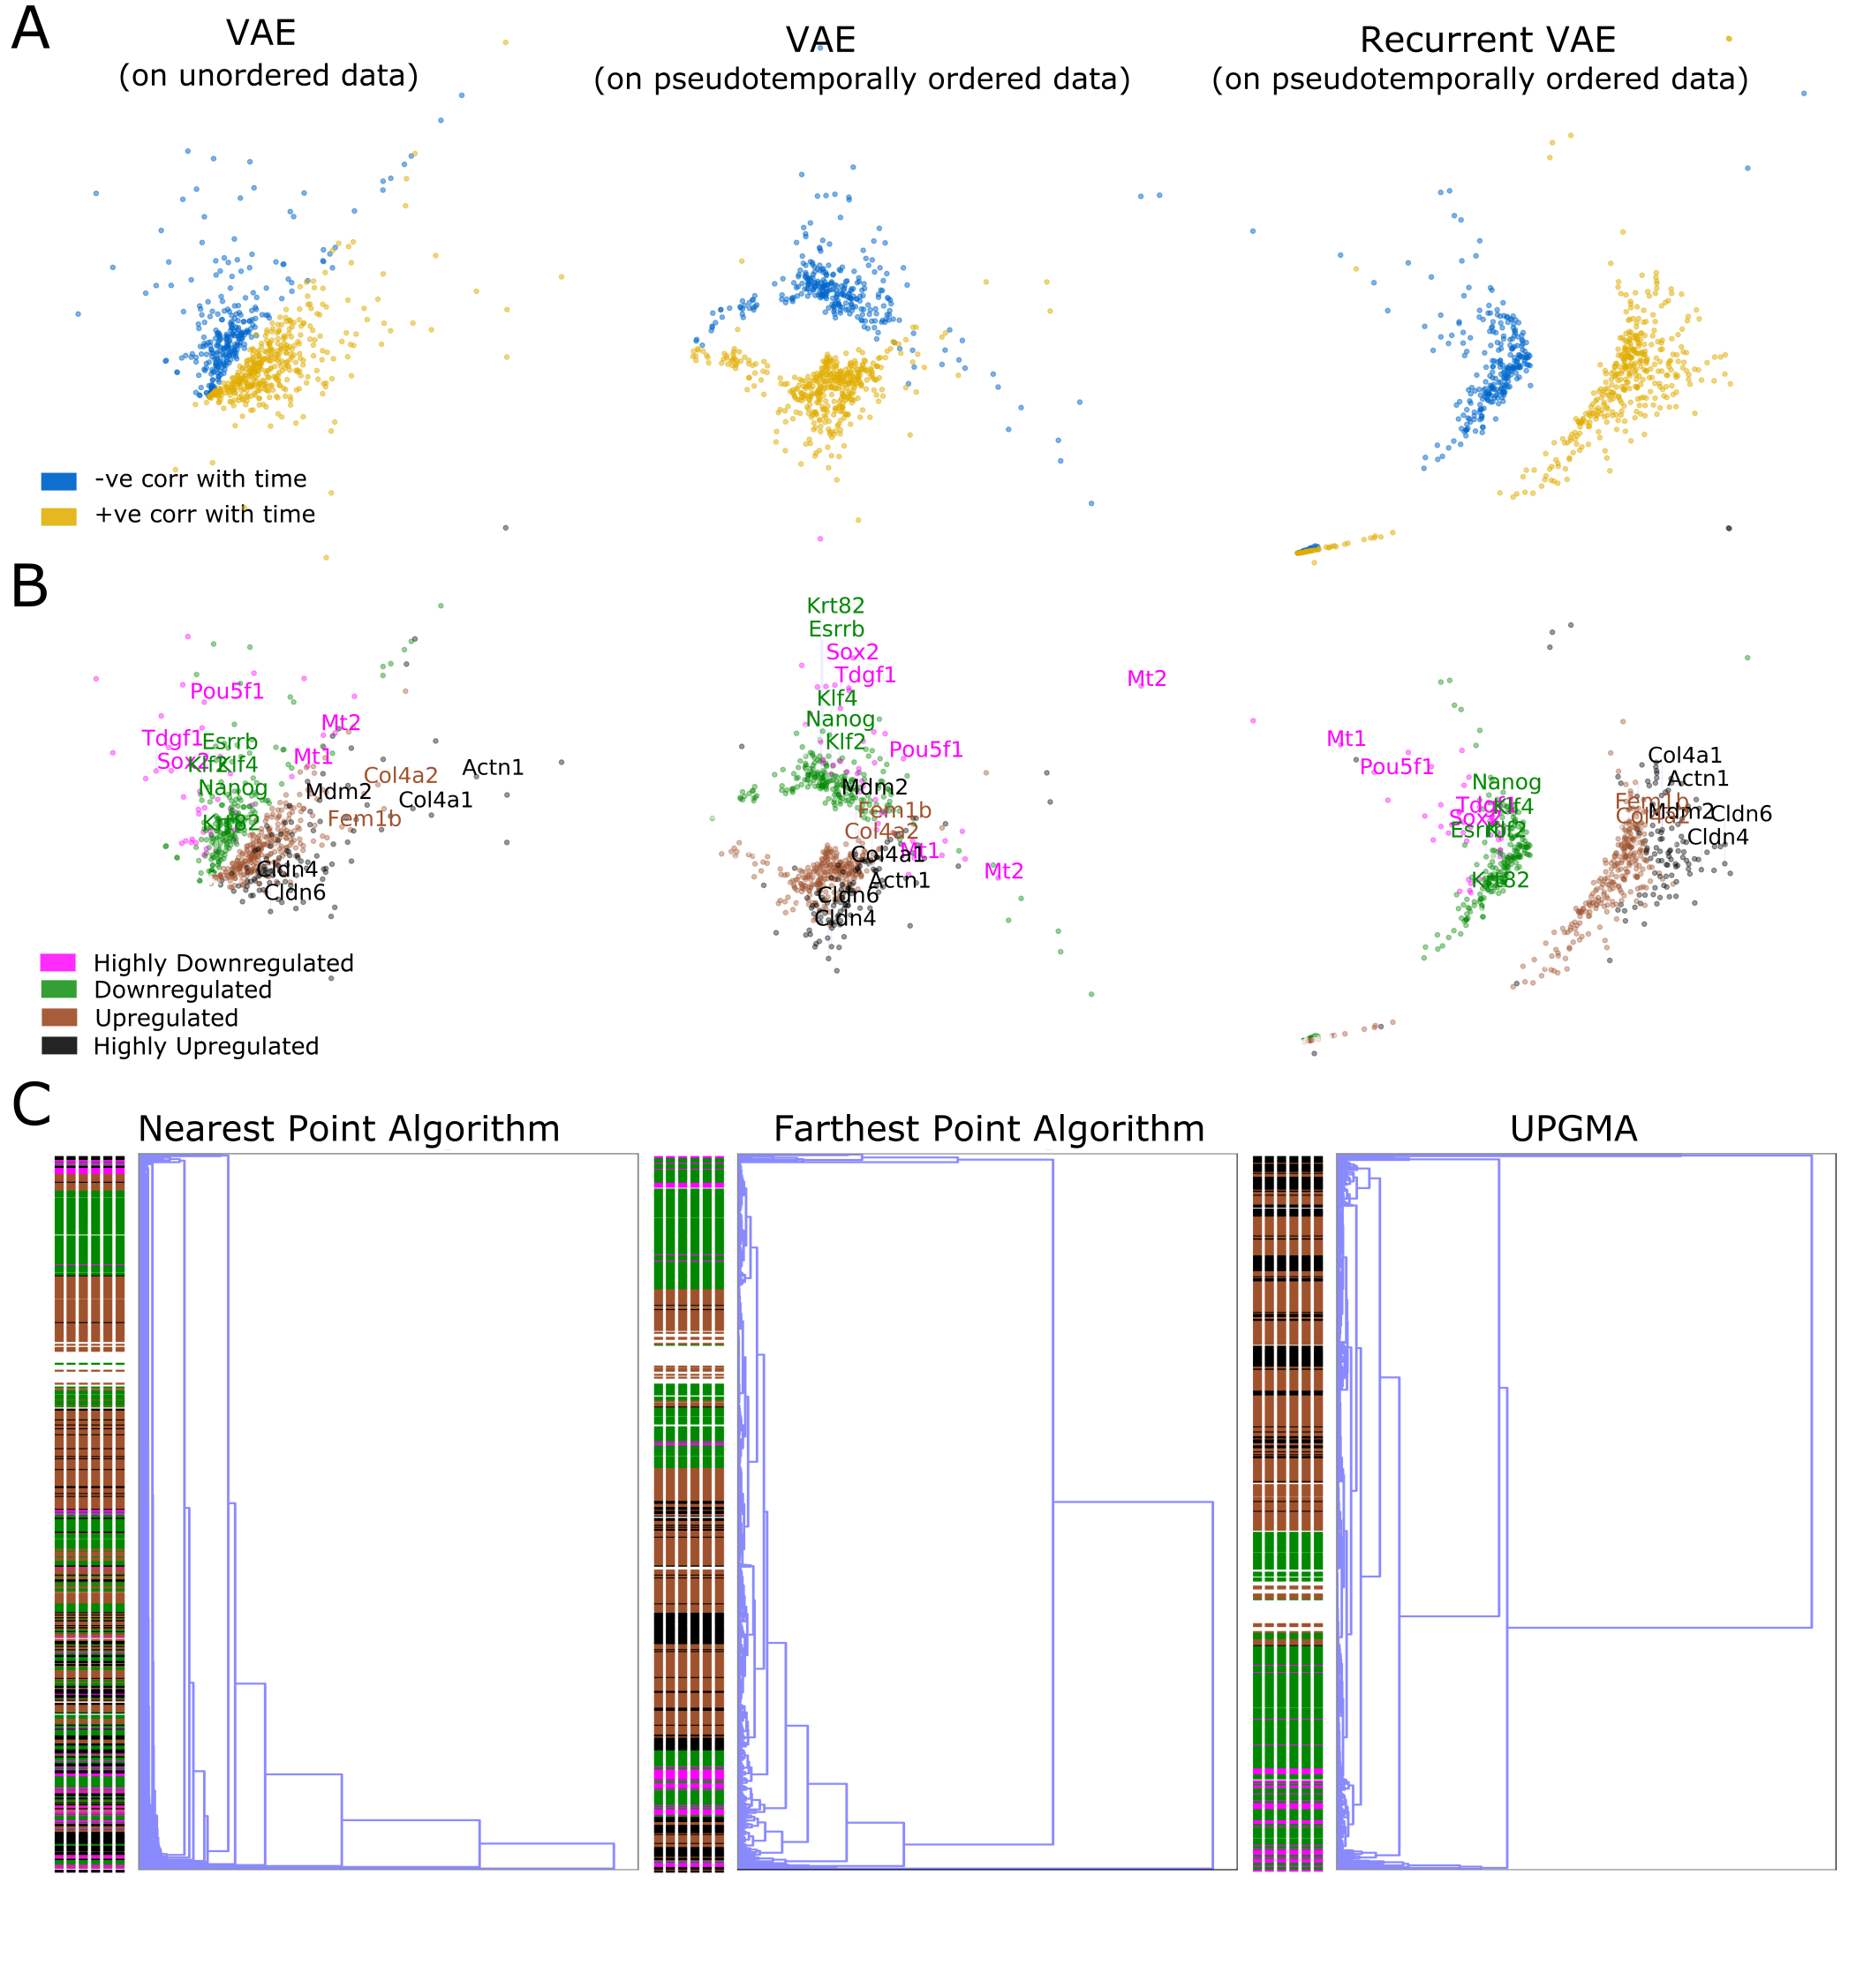
\includegraphics[width=\linewidth]{figures/vae_comp.png}
 % archetecture.png: 1149x508 px, 72dpi, 40.53x17.92 cm, bb=0 0 1149 508
    \caption[Comparison of information captured in RVAgene latent space compared to a standard fully connected VAE and results of standard hierarchical clusterings.]{\textbf{Comparison of information captured in RVAgene latent space compared to a standard fully connected VAE and results of standard hierarchical clusterings.}
    ({\bf A}) Here we show latent spaces learned by fully connected VAE and RVAgene. The pseudotemporally ordered data was also smoothed. ({\bf B}) We annotate the leanred latent spaces using the top 4 clusters detected by DPGP on this dataset. In all three of these cases we report best results after relevant hyperparameter search and optimal training. ({\bf C}) We perform standard hierarchical clusterings (Nearest Point Algorithm, Farthest Point Algorithm and UPGMA (Unweighted Pair Group Method with Arithmetic mean) ) on pseudotemporally ordered and smoothed ESC data and annotate the learned representation in the same manner as in (B).} 
  \label{fig:fig4}
\end{figure}}

{
To assess the ability of the model to reconstruct genes not used during training, we kept aside 300 genes for testing and trained RVAgene on the remaining 432 genes.
We note that in this case (and in the case of single-cell datasets in general), the generative model of RVAgene produces pseudotime-smoothed gene expression trajectories, rather than being generative of raw pseudotemporal data, which tend to display overall high noise levels.
}
Reconstructed test gene expression profiles are shown for three reconstructed genes (\hyperref[fig:fig3]{Fig. 2E}), chosen to sample across the spectrum of reconstruction errors (\hyperref[fig:fig3]{Fig. 2F}). The reconstruction for {\em Ddt}, which has a reconstruction error near the mode (\hyperref[fig:fig3]{Fig. 2F}), shows very high accuracy. The reconstruction for {\em Hmgb2}, which has twice the reconstruction error, still broadly captures the temporal profile but with lesser accuracy. Finally we show the reconstruction for {\em Rhox4e}, a gene that was sampled from the long tail of the reconstruction error distribution, i.e. does not well match the data. Comparing these three examples with the full distribution of reconstruction errors  (\hyperref[fig:fig3]{Fig. 2F}), we see that the large majority of genes lie to the left of {\em Hmgb2}, i.e. have better-than-moderate accuracy. The reconstruction error of {\em Hmgb2} is close to 0.005, which we use as a cut off for ``well-reconstructed'' genes, based on analysis of individual gene reconstructions. The cumulative reconstruction error distribution reiterates this point: 230 out of 300 genes (77\%) have a reconstruction error $\leq 0.005$ (\hyperref[fig:fig3]{Fig. 2G}); we can conclude that the majority of test genes were faithfully reconstructed by the model.
\par
RVAgene accurately reconstructed most gene profiles using only $\sim60 {\%}$ of the data for training (\hyperref[fig:fig3]{Fig. 2G}), likely due to co-regulation of gene expression programs. This led to a question: what is the smallest training gene set that can be used to accurately reconstruct gene dynamics? We subset the data randomly into train/test sets and trained separate RVAgene models on each. We found that reconstruction errors slowly increase as the size of the training set decreases, but not until the training set was as low as $18\%$ of the data did the reconstruction errors significantly increase (\hyperref[fig:fig3]{Fig. 2G}, \hyperref[supp]{Fig. S4}). Analysis of the cumulative distribution of reconstruction errors across all groups found that RVAgene reconstructs the majority of gene temporal profiles well (defined as below a reconstruction error of 0.005) if $\geq 45\%$ of the data is used for training. The successful reconstruction of gene expression dynamics de novo while training on  small subsets of the data suggests widespread co-regulation of gene expression programs during embryonic stem cell differentiation, as found in previous work \citep{jang2017dynamics}.
% This information is a useful indicator to whether an algorithm estimating number of clusters is overfitting or underfitting (i.e. detecting too many or too few clusters), we talk about this in more detail later in \hyperref[discussion1]{Discussion} section. 

%{\centering
%\begin{figure}
%  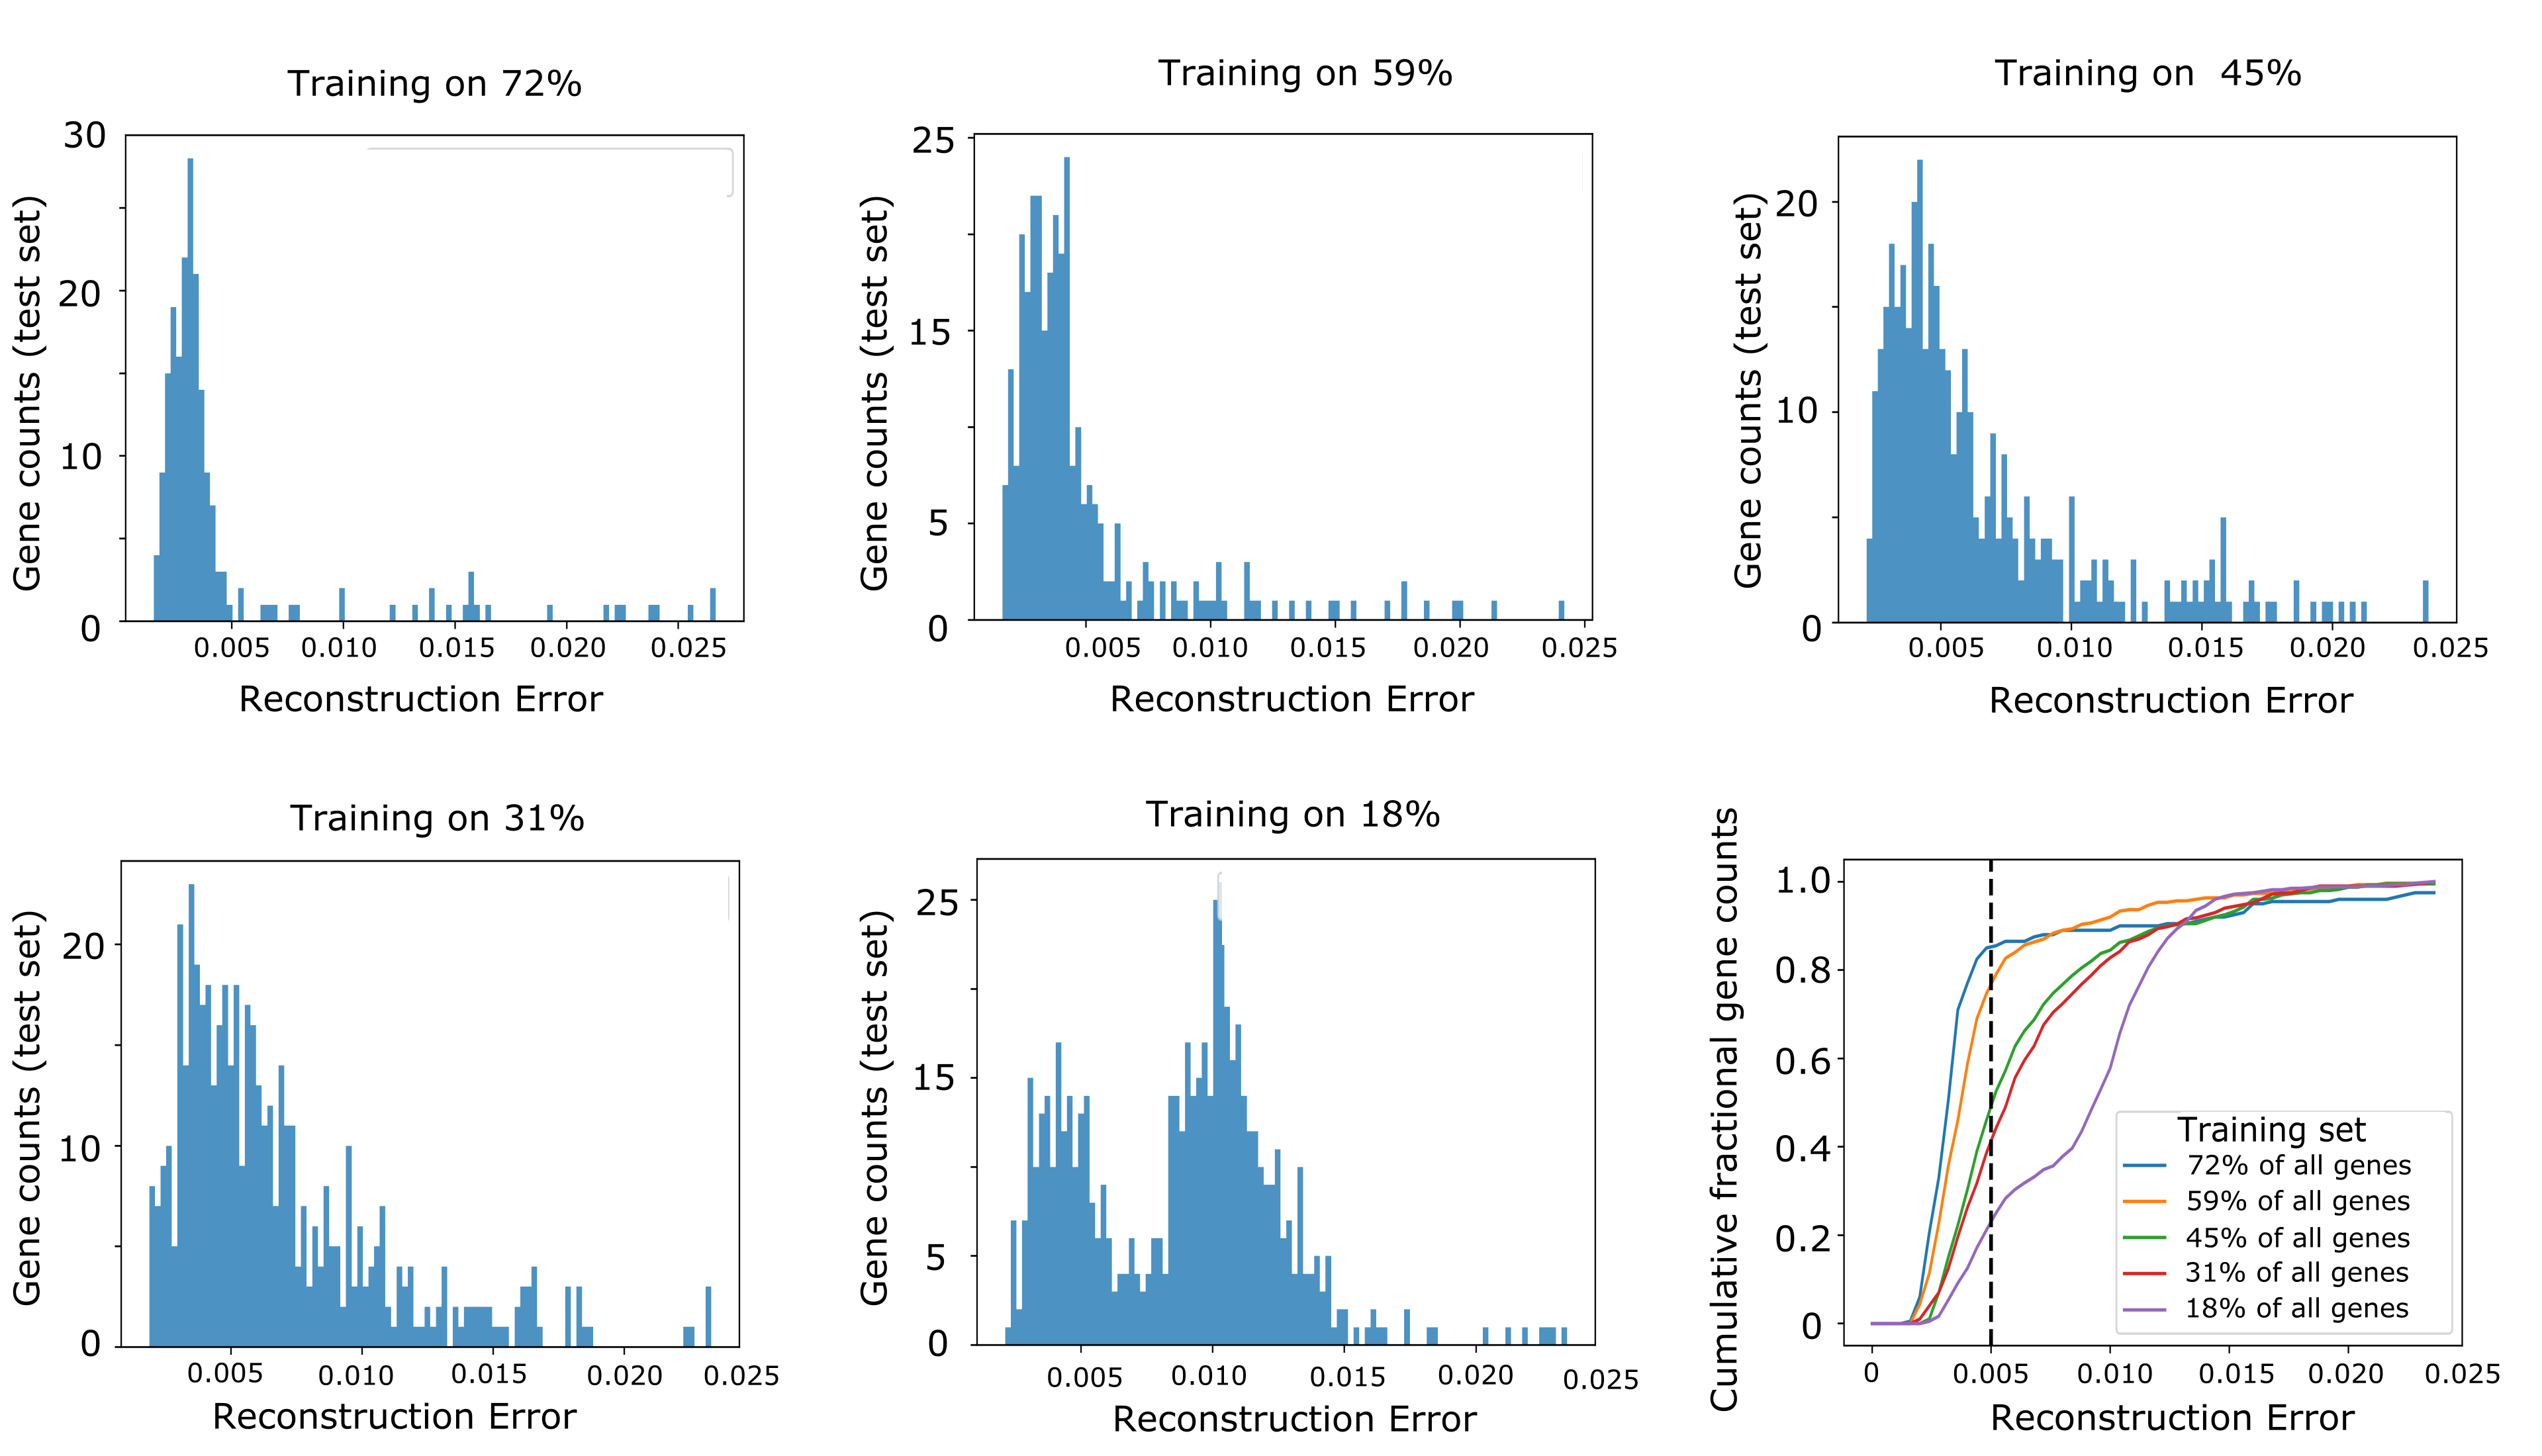
\includegraphics[width=\linewidth]{./figures/supp_varying_test_set_sizes.png}
 % archetecture.png: 1149x508 px, 72dpi, 40.53x17.92 cm, bb=0 0 1149 508
%    \caption{{\bf Accuracy of RVAgene reconstructions for different train/test group sizes.} Distributions of reconstruction errors on randomly sampled sets of test genes, where the full data were split into test groups of: 200 genes (train on 72\%), 300 genes (train on 59\%), 400 genes (train on 45\%), 500 genes (train on 31\%), and 600 genes (train on 18\%). Cumulative fractional distribution of reconstruction errors (cumulative count/test set size) for all groups.}
%  \label{fig:fig5}
%\end{figure}
%}

